\chapter[Systèmes d'équations]{Systèmes équations à plusieurs inconnues}



Nous avons déjà vu les équations à une seule inconnue. Intéressons-nous maintenant aux équations à plusieurs  inconnues.

Pour pouvoir déterminer de manière unique la valeur des inconnues, il faut que le nombre d'équations soit égal au nombre d'inconnues. Aussi durant ce chapitre, nous nous intéresserons  tout d'abord aux systèmes de deux équations à deux inconnues, puis aux systèmes de trois équations à trois inconnues.

\section{Systèmes $2\times 2$}

Essayons de trouver les valeurs de $x$ et de $y$ qui vérifient les deux équations suivantes en même temps :
$$
\left\{
\begin{array}{lll}
2x+3y &=& 8\\
4x-2y &=& 0
\end{array}
\right.
$$
\index{équation!à deux inconnues! premier degré}
Nous verrons ainsi trois méthodes différentes qui nous permettent de déterminer ces valeurs.

\subsection{Substitution}

Le principe de cette méthode est assez simple. En isolant une inconnue dans l'une des deux équations, puis en remplaçant cette inconnue dans l'autre, on se retrouve avec une équation à une inconnue que l'on sait résoudre. Ainsi dans l'exemple on a :
$$
\begin{array}{lr}
\left\{
\begin{array}{lll}
2x+3y &=& 8\\
4x-2y &=& 0
\end{array}
\right.
&(\mbox{ isoler }y\mbox{ dans la deuxième}) \\
\ssi \left\{
\begin{array}{lll}
2x+3y &=& 8\\
-2y &=& -4x
\end{array}
\right.
& \\
\ssi\left\{
\begin{array}{lll}
2x+3\textcolor{red}{y} &=& 8\\
\textcolor{red}{y} &=& \textcolor{red}{2x}
\end{array}
\right.
&(\mbox{remplacer }\textcolor{red}{y}\mbox{ par }\textcolor{red}{2x}\mbox{ dans la première})\\
\ssi\left\{
\begin{array}{lll}
2x+3 \cdot \textcolor{red}{2x} &=& 8\\
y &=& 2x
\end{array}
\right.
&(\mbox{résoudre la première})\\
\ssi\left\{
\begin{array}{lll}
8x &=& 8\\
y &=& 2x
\end{array}
\right.
&\\
\ssi\left\{
\begin{array}{lll}
x&=& 1\\
y &=& 2x
\end{array}
\right.
&(\mbox{remplacer }x\mbox{ par }1\mbox{ dans la deuxième})\\
\ssi\left\{
\begin{array}{lll}
x&=& 1\\
y &=& 2\cdot 1 = 2
\end{array}
\right. & \\
\end{array}
$$

Ainsi $x=1$ et $y=2$ et on note l'ensemble des solutions
$$
S=\left\{(1;2)\right\}.
$$

\subsection{Combinaison linéaire}

Cette méthode consiste, comme son nom l'indique, à combiner (c'est-à-dire additionner ou soustraire) deux équations pour supprimer une inconnue. Pour ce faire, il faut parfois commencer par multiplier l'une ou l'autre équation pour avoir le même nombre d'inconnues que l'on souhaite supprimer. Dans l'exemple :
$$
\begin{array}{lr}
\left\{
\begin{array}{lll}
2x+3y &=& 8\\
4x-2y &=& 0
\end{array}
\right.
&(\mbox{ multiplier par }2\mbox{ la première équation}) \\
\ssi 
\left\{
\begin{array}{lll}
4x+6y &=& 16\\
4x-2y &=& 0
\end{array}
\right.
&(\mbox{ soustraire la deuxième équation de la première}) \\
\Rightarrow
8y = 16
&(\mbox{ résoudre l'équation}) \\
\ssi
y = 2
&(\mbox{ reprendre le système de base}) \\
&\\
&\\
\left\{
\begin{array}{lll}
2x+3y &=& 8\\
4x-2y &=& 0
\end{array}
\right.
&(\mbox{ multiplier par }2\mbox{ la première et par }3\mbox{ la deuxième}) \\
\ssi
\left\{
\begin{array}{lll}
4x+6y &=& 16\\
12x-6y &=& 0
\end{array}
\right.
&(\mbox{ additionner les deux équations}) \\
\Rightarrow
16x = 16
&(\mbox{ résoudre l'équation}) \\
\ssi
x = 1
&(\mbox{ isoler }y\mbox{ dans la deuxième}) \\
\end{array}
$$

\subsection{Méthode de Cramer}

Gabriel Cramer\index{Cramer Gabriel}, né le 31 juillet 1704 à Genève et mort le 4 janvier 1752 à Bagnols-sur-Cèze, est un mathématicien suisse, professeur de mathématiques et de philosophie à l'académie de Genève.\footnote{Tiré explicitement de Wikipedia.com, consulté le 27 novembre 2015}

Il est notamment connu pour avoir donné une méthode générale de résolution des systèmes d'équations linéaires à plusieurs inconnues.

\begin{theoreme}
Soit un système linéaire de deux équations à deux inconnues du type
$$
\left\{
\begin{array}{lcl}
a_1 x + b_1 y &=& c_1\\
a_2 x + b_2 y &=& c_2
\end{array}
\right.
$$
Et soit les déterminants 
$$
\begin{array}{lcr}
D = \vaabs{\begin{array}{cc}
a_1 & b_1\\
a_2 & b_2
\end{array}},
&
D_x = \vaabs{\begin{array}{cc}
c_1 &b_1\\
c_2 & b_2
\end{array}},
&
D_y = \vaabs{\begin{array}{cc}
a_1 & c_1\\
a_2 & c_2
\end{array}}
\end{array}.
$$
Alors la réponse du système est donnée par
$$
x= \frac{D_x}{D} \mbox{ et } y = \frac{D_y}{D}
$$
\end{theoreme}

\begin{remarque}
Dans le théorème, l'ordre des colonnes est le suivant :
$$
AB,\quad CB,\quad AC
$$
Nous nous en rappellerons par la phrase suivante :
\textcolor{red}{À Bex, c'est bien assez !}
\end{remarque}

Pour calculer un déterminant, on utilise la règle suivante :
$$
\begin{array}{l}
\xymatrix{
a_1\ar@[blue][rd] & b_1\ar@[red][ld] \\
a_2 & b_2 }
\end{array}
= \textcolor{blue}{a_1 \cdot b_2} - \textcolor{red}{b_1 \cdot a_2}
$$

\begin{exemple}
Toujours pour notre système 
$$
\left\{
\begin{array}{lll}
2x+3y &=& 8\\
4x-2y &=& 0
\end{array}
\right.
$$
On a 
$$
A = \left(\begin{array}{c}2 \\ 4 \end{array} \right),\quad
B = \left(\begin{array}{c}3 \\ -2 \end{array} \right),\quad
C = \left(\begin{array}{c}8 \\ 0 \end{array} \right).
$$

Ainsi 
$$
\begin{array}{l}
D = \vaabs{AB} = \vaabs{\begin{array}{cc}
2 & 3 \\
4 & -2
\end{array}}
= 2\cdot (-2) - 3\cdot 4 = -16
\\
D_x = \vaabs{CB} = \vaabs{\begin{array}{cc}
8 & 3 \\
0 & -2
\end{array}}
= 8\cdot (-2) - 3\cdot 0 = -16
\\
D_y = \vaabs{AC} = \vaabs{\begin{array}{cc}
2 & 8 \\
4 & 0
\end{array}}
= 2\cdot 0 - 8\cdot 4 = -32
\end{array}
$$

Donc 
$$
x = \frac{D_x}{D} = \frac{-16}{-16}= 1 \mbox{ et } y = \frac{D_y}{D} = \frac{-32}{-16}= 2.
$$
\end{exemple}

\section{Systèmes $3\times 3$}


Essayons de trouver les valeurs de $x$ , de $y$ et de $z$ qui vérifient les trois équations suivantes en même temps :
$$
\left\{
\begin{array}{lll}
2x-y+3z &=& 7\\
x-2y+4z &=& 3\\
3x-7y+8z &=& 3
\end{array}
\right.
$$
\index{équation!à trois inconnues! premier degré}
Nous verrons ainsi deux méthodes différentes qui nous permettent de déterminer ces valeurs.

\subsection{Combinaison linéaire}

Cette méthode est identique à celle employée pour les systèmes $2\times 2$. Elle consiste, par multiplication et soustraction/addition, à se ramener à un système $2\times 2$ que l'on sait résoudre. Ainsi :
$$
\begin{array}{c}

\left\{
\begin{array}{llll}
2x-y+3z &=& 7 &(A)\\
x-2y+4z &=& 3 &(B)\\
3x-7y+8z &=& 3 & (C)
\end{array}
\right.
\\
\\
\begin{array}{cc}
(A)-2\cdot (B)&
(C)-3\cdot(B)\\
&\\
\begin{array}{rrrrrr}
2x & -y &+3z &=&7&\\
-2x &+4y &-8z&=&-6&\\
\hline
&3y&-5z&=&1 &(D)\\
\end{array}
&
\begin{array}{rrrrrr}
3x & -7y & +8z &=& 3&\\
-3x & +6y & -12z &=& -9&\\
\hline
&-y&-4z &=& -6&(E)\\
\end{array}\\
\end{array}
\\
\\
\ssi \left\{
\begin{array}{rrrrrr}
x&-2y&+4z &=& 3 &(B)\\
&3y&-5z&=&1 &(D)\\
&-y&-4z &=& -6&(E)\\
\end{array}
\right.
\\
\begin{array}{cc}
3\cdot (E) & (D)+(F)\\
&\\
\ssi \left\{
\begin{array}{rrrrrr}
x&-2y&+4z &=& 3 &(B)\\
&3y&-5z&=&1 &(D)\\
&-3y&-12z &=& -18&(F)\\
\end{array}
\right.
& \ssi \left\{
\begin{array}{rrrrrr}
x&-2y&+4z &=& 3 &\\
&3y&-5z&=&1 &\\
&&-17z &=& -17&\\
\end{array}
\right.\\
&\\
&\\
&\mbox{remplacer en remontant}\\
&\\
\ssi \left\{
\begin{array}{rrrrrr}
x&-2y&+4z &=& 3 &\\
&3y&-5z&=&1 &\\
&&z &=& 1&\\
\end{array}
\right.
&
\ssi \left\{
\begin{array}{rrrrrr}
x&-2y&+4 &=& 3 &\\
&3y&-5&=&1 &\\
&&z &=& 1&\\
\end{array}
\right.\\
&\\
\ssi \left\{
\begin{array}{rrrrrr}
x&-2y&+4 &=& 3 &\\
&y&&=&2 &\\
&&z &=& 1&\\
\end{array}
\right.
&
\ssi \left\{
\begin{array}{rrrrrr}
x&-4&+4z &=& 3 &\\
&y&&=&2 &\\
&&z &=& 1&\\
\end{array}
\right.\\
\end{array}\\
\ssi \left\{
\begin{array}{rrrrrr}
x&& &=& 3 &\\
&y&&=&2 &\\
&&z &=& 1&\\
\end{array}
\right.\\
\end{array}
$$

On trouve donc l'ensemble des solutions :
$$
S=\{(3;2;1\}.
$$

\subsection{Méthode de Sarrus}

La méthode de Sarrus~\index{Sarrus} est aux systèmes $3\times 3$ ce que la méthode de Cramer est aux systèmes $2\times 2$. Ainsi 

\begin{theoreme}
Le système linéaire de trois équations à  trois inconnues du type
$$
\left\{
\begin{array}{rrrcr}
a_1 x & +b_1 y & + c_1 z &=&d_1\\
a_2 x & +b_2 y & + c_2 z &=&d_2\\
a_3 x & +b_3 y & + c_3 z &=&d_3\\
\end{array}
\right.
$$
admet les solutions
$$
x= \frac{D_x}{D}, \quad y=\frac{D_y}{D}, \quad z = \frac{D_z}{D},
$$
où $D$ est le déterminant $ABC$, $D_x$ le déterminant $DBC$, $D_y$ le déterminant $ADC$ et $D_z$ le déterminant $ABD$.
\end{theoreme}

Il nous reste maintenant à savoir comment on calcule un déterminant $3\times 3$. Il existe  une manière générale de calculer un déterminant $n\times n$ (et de même une manière de donner les solutions d'un système $n\times n$), mais elle est assez complexe. Nous verrons donc la solution "simplifiée" :

Dans notre exemple, le déterminant que l'on doit chercher est
$$
D=
\vaabs{
\begin{array}{ccc}
2&-1&3\\
1&-2&4\\
3&-7&8
\end{array}
}
$$
On commence par répéter les deux premières colonnes à droite, puis on utilise les flèches pour calculer sa valeur :
$$D=
\begin{array}{c}
\xymatrix{
2\ar@[blue][rd]&-1\ar@[blue][rd]&3\ar@[blue][rd] \ar@[red][ld]&2\ar@[red][ld]&-1\ar@[red][ld]\\
1&-2\ar@[blue][rd]\ar@[red][ld]&4\ar@[blue][rd]\ar@[red][ld]&1\ar@[blue][rd]\ar@[red][ld]&-2\\
3&-7&8&3&-7\\
}\\
\\
= \textcolor{blue}{2 \cdot (-2) \cdot 8 + (-1)\cdot 4 \cdot 3 + 3\cdot 1  \cdot(-7)} \textcolor{red}{-3\cdot (-2)\cdot 3 -2\cdot 4 \cdot (-7) - (-1)\cdot 1 \cdot 8}\\
= 17\\
\end{array}
$$

De la même manière, on trouve : $D_x = 51$, $D_y = 34$ et $D_z = 17$ et on obtient bien l'ensemble des solutions
$$
S = \{(3;2;1)\}
$$

\section{Interprétation géométrique}

Dans le chapitre~\ref{droite_plan}, nous avons vu qu'une droite est représentée par son équation implicite
$$
ax+by=c.
$$
Aussi, résoudre un système d'équation $2\times 2$ revient à dessiner les deux droites et à trouver leur point d'intersection. Si l'on reprend l'exemple 
$$
\left\{
\begin{array}{lll}
2x+3y &=& 8\\
4x-2y &=& 0
\end{array}
\right.
$$
on a la représentation suivante :

\begin{center}
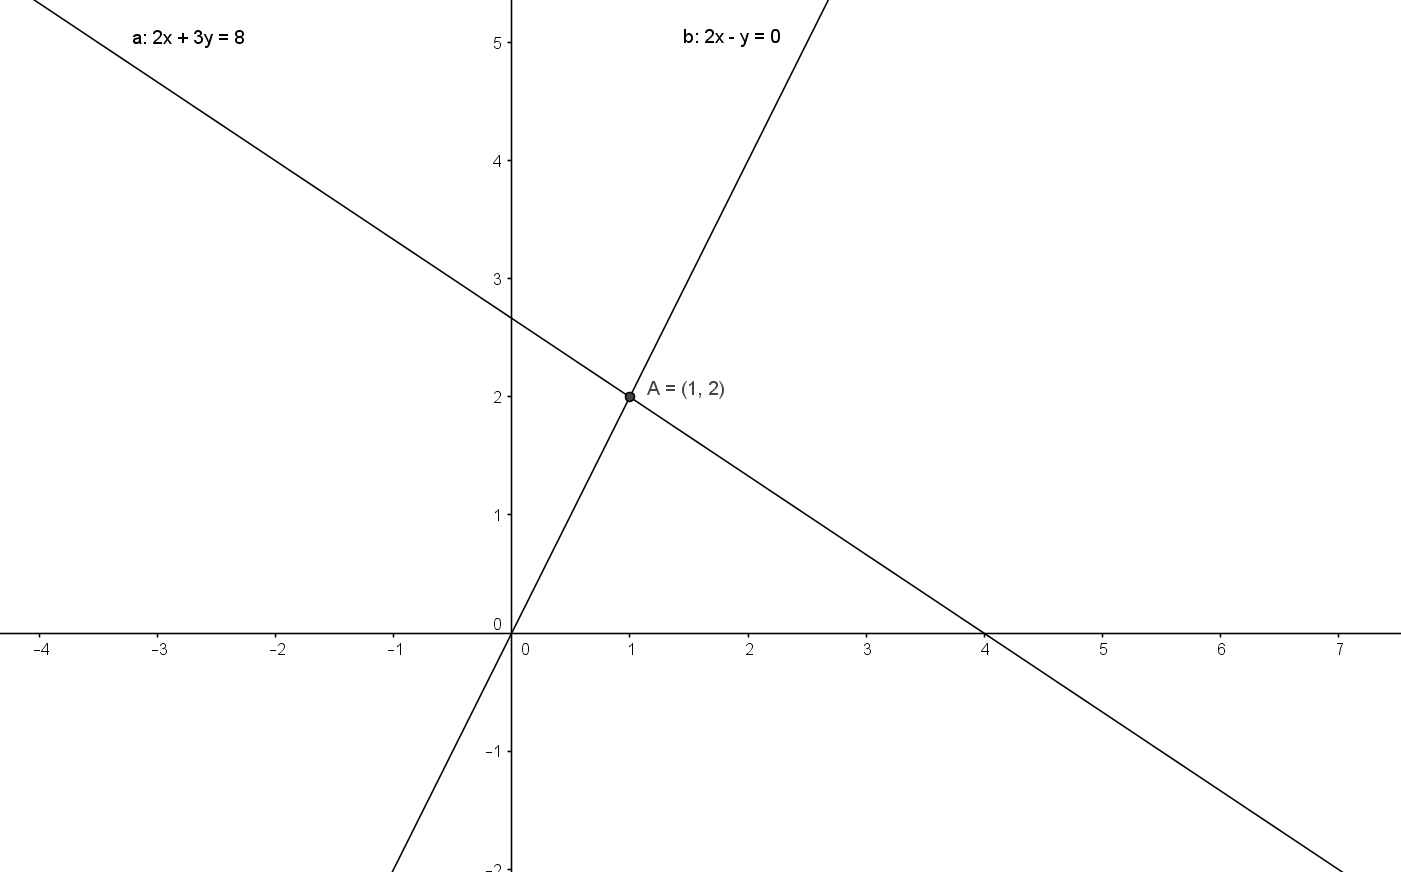
\includegraphics[width = 0.9 \textwidth]{systeme/systeme2x2.png}
\end{center}

De même, on peut représenter un système $3\times 3$ dans l'espace. Chaque équation correspond à un plan, et la solution se trouve à l'intersection des trois plans :

\begin{center}
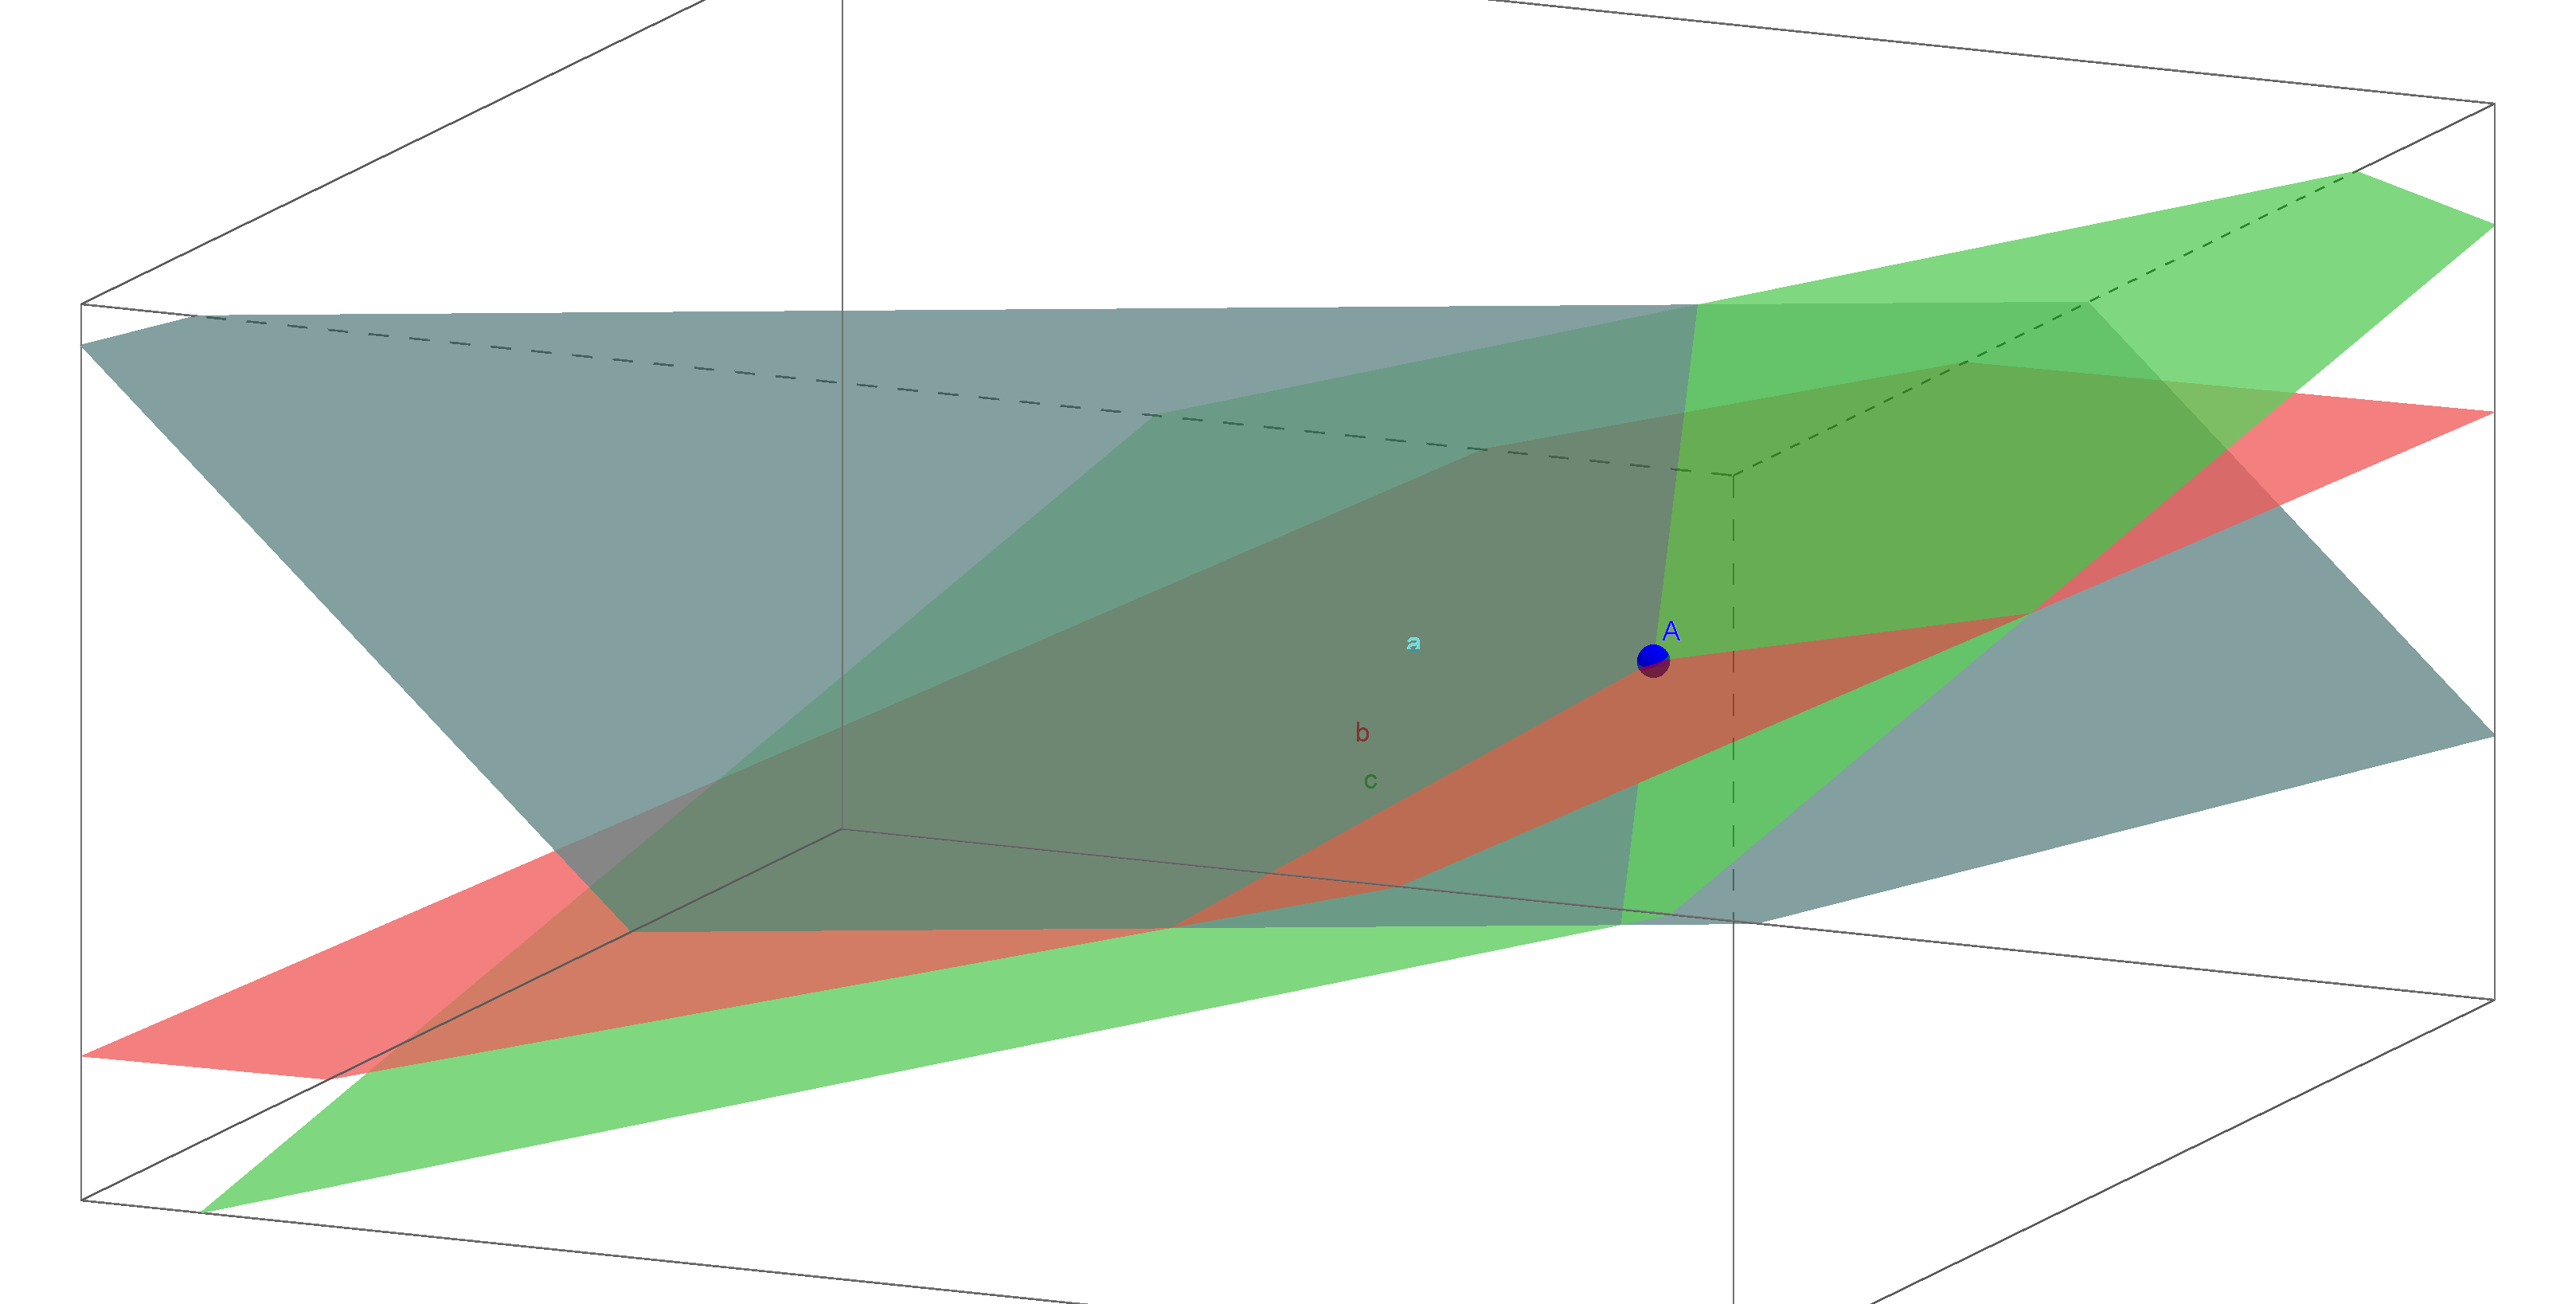
\includegraphics[width = 0.9 \textwidth]{systeme/systeme3x3.png}
\end{center}

On peut généraliser de la sorte aux systèmes $4\times 4$, $5\times 5$, etc. mais ça devient vite très compliqué à représenter.
\section{Exercice}

\subsection{Systèmes $2\times 2$}

\begin{exercice}
Résoudre les systèmes suivants :
\begin{multicols}{2}
\begin{enumerate}
\item $$\left\{ \begin{array} {l}
    3x+4y=24 \\ 
   5y=15 \\ 
\end{array} \right.$$ 
\item $$\left\{ \begin{array} {l}
    x+y=19 \\ 
   2x-y=2 \\ 
\end{array} \right.$$ 
\item $$\left\{ \begin{array} {l}
    12x-5y=29 \\ 
   4x-3y=11 \\ 
\end{array} \right.$$ 
\item $$\left\{ \begin{array} {l}
    x+y=28 \\ 
   3x-11y=8y-48 \\ 
\end{array} \right.$$ 
\item $$\left\{ \begin{array} {l}
    x+2y=22 \\ 
   5(x-5)=y-3 \\ 
\end{array} \right.$$ 
\item $$\left\{ \begin{array} {l}
    x-12y=4 \\ 
   41y+7=3x \\ 
\end{array} \right.$$ 
\item $$\left\{ \begin{array} {l}
    x+3y=11 \\ 
   5y-68=3(x-1) \\ 
\end{array} \right.$$ 
\item $$\left\{ \begin{array} {l}
    12x-5y=57 \\ 
   15y+2x=19 \\ 
\end{array} \right.$$ 
\item $$\left\{ \begin{array} {l}
    24x+7y=69 \\ 
   7(9x-5y)=21 \\ 
\end{array} \right.$$ 
\item $$\left\{ \begin{array} {l}
    8x-9y=53 \\ 
   5x+18y=41 \\ 
\end{array} \right.$$ 
\item $$\left\{ \begin{array} {l}
    5x=y \\ 
   12x-2y=10 \\ 
\end{array} \right.$$
\item $$\left\{ \begin{array} {l}
    2x+3y=4 \\ 
   3y+10x=44 \\ 
\end{array} \right.$$
\item $$\left\{ \begin{array} {l}
    2x-3y+35=0 \\ 
   4x-y-25=0 \\ 
\end{array} \right.$$
\item $$\left\{ \begin{array} {l}
    12x+11y=6 \\ 
   3y-2x=28 \\ 
\end{array} \right.$$
\item $$\left\{ \begin{array} {l}
    2x+5y=69 \\ 
   y-4(x-7)=67-3x \\ 
\end{array} \right.$$
\item $$\left\{ \begin{array} {l}
    72x+14y=330 \\ 
   63x+7y=273 \\ 
\end{array} \right.$$
\item $$\left\{ \begin{array} {l}
    21x+8y+66=0 \\ 
   28x-23y-13=0 \\ 
\end{array} \right.$$
\item $$\left\{ \begin{array} {l}
    3y-4x=1 \\ 
   6(2x+y)=17 \\ 
\end{array} \right.$$
\item $$\left\{ \begin{array} {l}
    123x-234y=-99 \\ 
   345x-456y=123 \\ 
\end{array} \right.$$
\item $$\left\{ \begin{array} {l}
    999x+y=1001 \\ 
   x+999y=1999 \\ 
\end{array} \right.$$
\end{enumerate}
\end{multicols}
\end{exercice}

\begin{exercice} 
Résoudre les systèmes suivants :
\begin{multicols}{2}
\begin{enumerate}
\item $$\left\{ \begin{array} {l}
    x+\frac{3y}{7}=17 \\ 
   y-\frac{5x}{8}=16 \\ 
\end{array} \right.$$ 
\item $$\left\{ \begin{array} {l}
    \frac{x}{3}+\frac{y}{4}=9 \\ 
   \frac{x}{4}+\frac{y}{5}=7 \\ 
\end{array} \right.$$ 
\item $$\left\{ \begin{array} {l}
    \frac{4x-5}{2y-3}=3 \\ 
   \frac{3x+5}{y+1}=4 \\ 
\end{array} \right.$$ 
\item $$\left\{ \begin{array} {l}
    \frac{x-1}{8}+\frac{y-2}{5}=2 \\ 
   2x+\frac{2y-5}{3}=21 \\ 
\end{array} \right.$$ 
\item $$\left\{ \begin{array} {l}
    \frac{x-4}{3}-\frac{3y+4}{10}=x-y \\ 
   \frac{2x-5}{5}-\frac{2y-4}{4}=x-12 \\ 
\end{array} \right.$$ 
\item $$\left\{ \begin{array} {l}
    \frac{4x+15}{3}-\frac{3y-5}{5}=x \\ 
   \frac{2y+3x}{4}+\frac{y+15}{5}=y \\ 
\end{array} \right.$$
\item $$\left\{ \begin{array} {l}
    \frac{x-y}{3}-\frac{1}{4}\left( x-\frac{10-2y}{3} \right)=3 \\ 
   \frac{x-5y}{5}+\frac{x+2}{2}=x-4 \\ 
\end{array} \right.$$
\item $$\left\{ \begin{array} {l}
    \frac{3x}{5}+\frac{4y}{10}=\frac{x-y}{5} \\ 
   \frac{10(2x+3)}{11}-2\left( y-\frac{3x-5}{8} \right)=60 \\ 
\end{array} \right.$$
\item $$\left\{ \begin{array} {l}
    \frac{13}{3+x+2y}+\frac{3}{6+4x-5y}=0 \\ 
   \frac{6x-5y+4}{3}=\frac{3x+2y+1}{19} \\ 
\end{array} \right.$$
\item $$\left\{ \begin{array} {l}
    \frac{x+5}{x+1}=\frac{y-9}{y+7}+\frac{112}{(x+1)(y+7)} \\ 
   2x+10=3y+1 \\ 
\end{array} \right.$$
\end{enumerate}
\end{multicols}
\end{exercice}

\subsection{Systèmes $n\times n$}

\begin{exercice}
Résoudre les systèmes suivants (algorithme de Gauss-Jordan) : 
\begin{multicols}{2}
\begin{enumerate}
\item $$\left\{ \begin{array}{l}
    4x+3y+6z=41 \\ 
   8x+5y=31 \\ 
   7y=21 \\ 
\end{array} \right.$$

\item $$\left\{ \begin{array}{l}
    2x-3y+2z=41 \\ 
   5x+3y+z=10 \\ 
   9x=27 \\ 
\end{array} \right.$$

\item $$\left\{ \begin{array}{l}
    7x-4y-5z=56 \\ 
   3y-2z=13 \\ 
   5x-3y=22 \\ 
\end{array} \right.$$

\item $$\left\{ \begin{array}{l}
    6x-y+3z=38 \\ 
   5x-2y+z=24 \\ 
   3x-y+5z=24 \\ 
\end{array} \right.$$

\item $$\left\{ \begin{array}{l}
    x+y+z=25 \\ 
   x-y+z=5 \\ 
   x+2z=2y-10 \\ 
\end{array} \right.$$

\item $$\left\{ \begin{array}{l}
    x-y-z=6 \\ 
   x-2y-3z=10 \\ 
   5x+6y+z=2 \\ 
\end{array} \right.$$

\item $$\left\{ \begin{array}{l}
    -x-2y+3z=18 \\ 
   -2x+2y+3z=36 \\ 
   5x+2y-z=10 \\ 
\end{array} \right.$$

\item $$\left\{ \begin{array}{l}
    3x-y+z=29 \\ 
   x+3y+30z=6 \\ 
   x-y+z=17 \\ 
\end{array} \right.$$ 
\end{enumerate}
\end{multicols}
\end{exercice}

\begin{exercice}
Résoudre les systèmes suivants (méthode des déterminants, règle de Sarrus) : 
\begin{multicols}{2}
\begin{enumerate}
\item $$\left\{ \begin{array}{l}
    2x+3y+4z=53 \\ 
   3x+5y-4z=2 \\ 
   4x+7y-2z=31 \\ 
\end{array} \right.$$

\item $$\left\{ \begin{array}{l}
    4x+5y-3z=-1 \\ 
   2x-10y+z=2 \\ 
   -3x+15y+4z=8 \\ 
\end{array} \right.$$
\item $$\left\{ \begin{array}{l}
    14x-13y+12z=61 \\ 
   -11x+15y+18z=168 \\ 
   10x+17y-16z=3 \\ 
\end{array} \right.$$

\item $$\left\{ \begin{array}{l}
    15x-13y+18z=-45 \\ 
   17x+21y-31z=206 \\ 
   10x+12y-2z=40 \\ 
\end{array} \right.$$ 
\end{enumerate}
\end{multicols}
\end{exercice}

\begin{exercice}
Résoudre les systèmes suivants : 
\begin{multicols}{2}
\begin{enumerate}
\item $$\left\{ \begin{array}{l}
    x-\frac{4y-3}{3}+\frac{z-2}{2}=2 \\ 
   \frac{x}{5}-\frac{3y}{2}+3z=22 \\ 
   \frac{x-1}{4}-\frac{y-1}{5}=\frac{z-10}{10} \\ 
\end{array} \right.$$

\item $$\left\{ \begin{array}{l}
    \frac{4x-7}{3}-\frac{2(y-2)}{3}=z \\ 
   \frac{3x}{7}+\frac{2y-1}{7}-5z=1 \\ 
   \frac{2x+y}{5}+\frac{z}{4}=\frac{21}{4} \\ 
\end{array} \right.$$
 

\item $$\left\{ \begin{array}{l}
    \frac{x+2y-3z}{13}-4z=3(x+2) \\ 
   \frac{5x-1}{7}+2y-z=33 \\ 
   x+\frac{2y+7}{5}-z=3x-7 \\ 
\end{array} \right.$$

\item $$\left\{ \begin{array}{l}
    x+y+z=a+b \\ 
   \frac{1}{x-y}=\frac{1}{2b} \\ 
   \frac{x}{y-z}-\frac{1}{2}=\frac{b}{a-b} \\ 
\end{array} \right.$$ 
\end{enumerate}
\end{multicols}
\end{exercice}

\begin{exercice}
Résoudre les systèmes suivants avec des artifices de calcul : 
\begin{multicols}{2}
\begin{enumerate}
\item $$\left\{ \begin{array}{l}
    x+y=10 \\ 
   x+z=19 \\ 
   y+z=23 \\ 
\end{array} \right.$$

\item $$\left\{ \begin{array}{l}
    x+y+z=3 \\ 
   y+z+v=-2 \\ 
   x+z+v=6 \\ 
   x+y+v=2 \\ 
\end{array} \right.$$

\item $$\left\{ \begin{array}{l}
    -2x+y+z+v=-1 \\ 
   x-2y+z+v=11 \\ 
   x+y-2z+v=5 \\ 
   x+y+z-2v=17 \\ 
\end{array} \right.$$

\item $$\left\{ \begin{array}{l}
    x+y-z=17 \\ 
   x-y+z=13 \\ 
   -x+y+z=7 \\ 
\end{array} \right.$$

\item $$\left\{ \begin{array}{l}
    \frac{1}{x}+\frac{1}{y}=\frac{9}{20} \\ 
   \frac{1}{y}+\frac{1}{z}=\frac{13}{15} \\ 
   \frac{1}{x}+\frac{1}{z}=\frac{11}{12} \\ 
\end{array} \right.$$

\item $$\left\{ \begin{array}{l}
    x+y=18 \\ 
   y+z=14 \\ 
   z+u=10 \\ 
   u+v=6 \\ 
   x+v=12 \\ 
\end{array} \right.$$
\end{enumerate}
\end{multicols}
\end{exercice}

\subsection{Problèmes}

\begin{exercice}
Comment peut-on payer la somme de Fr. 99.— avec 27 pièces, les unes de Fr. 5.— les autres de Fr. 2.— ?
\end{exercice}

\begin{exercice}
Il y a 4 ans, l’âge d’un père était le quadruple de celui de son fils; dans 10 ans, il n’en sera plus que le double. Quels sont les âges actuels ?
\end{exercice}

\begin{exercice}
Il y a 7 ans, la moitié de l’âge de mon oncle surpassait le mien de 2 ans. Aujourd’hui mon âge surpasse de 5 ans les $\frac{2}{5}$ de celui de mon oncle. Quels sont les âges ?
\end{exercice}

\begin{exercice}
Deux sommes placées l’une à $4 \%$ et l’autre à $5 \%$ produisent ensemble un revenu annuel de Fr. 400.—. Si l’une était placée au taux de l’autre et inversement, elles donneraient alors Fr. 410.—. Quelles sont ces deux sommes ?
\end{exercice}

\begin{exercice}
Deux sommes placées à $5 \%$ donnent Fr. 550.— d’intérêts par an; en diminuant le taux de la première et en augmentant celui de la seconde, chacun de $\frac{1}{4} \%$, l’intérêt serait augmenté de Fr. 2.50. Quelles sont les deux sommes ?
\end{exercice}

\begin{exercice}
Deux sommes, l’une de Fr. 5’000.— et l’autre de Fr. 6’000.—, rapportent ensemble Fr. 525.— par an. En plaçant l’une au taux de l’autre et inversement, l’intérêt ne serait que de Fr. 520.—. Quels sont les deux taux ?
\end{exercice}

\begin{exercice}
Deux capitaux A et B ont été placés comme il suit: le $\frac{1}{4}$ de A et les $\frac{3}{5}$ de B à $4 \%$; les restes à $5  \%$. Le premier placement donne Fr. 2’160.— d’intérêts simples en 3 ans et l’autre Fr. 5’200.— en 4 ans. Trouver les deux capitaux.
\end{exercice}

\begin{exercice}
Jean à placé Fr. 12’600.— de plus que Louis et à $1 \%$ de plus; aussi retire-t-il Fr. 730.— d’intérêts de plus par an. Julien place Fr. 3’000.— de plus que Louis et à $2 \%$ de plus; son revenu annuel surpasse de Fr. 380.— celui de Louis. Déterminer les capitaux placés et les taux.
\end{exercice}

\begin{exercice}
Deux capitaux ont comme somme Fr. 6’000.—. Le 1er est placé à $1 \%$ de plus que le 2e et ils produisent ensemble Fr. 264.— d’intérêts par an. Si le premier était placé au taux du second, et réciproquement, ils produiraient Fr. 276.— d’intérêts. Quelles sont les deux sommes et à quels taux sont-elles placées ?
\end{exercice}

\begin{exercice}
Une somme d’argent a été partagée également entre un certain nombre de personnes. S’il y avait eu 6 personnes de plus, chacun eût reçu Fr. 2.— de moins. Au contraire, s’il avait eu 3 personnes de moins, chacune aurait reçu Fr. 2.— de plus. Déterminer le nombre de personnes, la part de chacun et la somme partagée.
\end{exercice}

\begin{exercice}
Un contremaître distribue une gratification à ses ouvriers; quand chaque ouvrier prend Fr. 1’400.— il ne reste plus que Fr. 700.—; mais si chaque ouvrier prenait Fr. 1’500.— il manquerait Fr. 2’600.—. Quel est le montant de cette gratification et combien y a-t-il d’ouvriers ?
\end{exercice}

\begin{exercice}
Jean-Paul dit à son camarade : “ Donne-moi 5 de tes billes et nous en auront autant l’un que l’autre ”. L’autre répond : “ Donne-moi 10 de tes billes et j’en aurai alors le double de ce qu’il te restera ”. Combien ont-ils de billes chacun ?
\end{exercice}

\begin{exercice}
En ajoutant 36 à un nombre de deux chiffres, on obtient le nombre renversé ; le chiffre des dizaines augmenté de 2, vaut les $\frac{3}{4}$ du chiffre des unités. Quel est ce nombre ?
\end{exercice}

\begin{exercice}
Un nombre de deux chiffres est tel qu’en y ajoutant 9, on obtient le nombre renversé et qu’en le diminuant de 9, le reste égale 4 fois la somme des chiffres. Quel est ce nombre ?
\end{exercice}

\begin{exercice}
On demandait à quelqu’un son âge, ainsi que celui de son père et de son grand-père. Il répondit : mon âge et celui de mon père font ensemble 56 ans; mon père et mon grand-père ont ensemble 100  ans, enfin mon âge et celui de mon grand-père font ensemble 80 ans. Déterminer les trois âges.
\end{exercice}

\begin{exercice}
Trois artilleurs A, B, C ont tiré des coups de canon. A et B ont tiré ensemble 20 coups de plus que C ; B et C, 32 coups de plus que A ; A et C, 28 coups de plus que B. Calculer le nombre de coups tirés par chaque artilleur.
\end{exercice}

\begin{exercice}
Un nombre de trois chiffres a 16 pour somme de ses chiffres ; en y ajoutant le nombre renversé, on obtient 1211; en retranchant du nombre le nombre renversé, on obtient 297. Quel est ce nombre ?
\end{exercice}

\section{Corrigés}

\subsection{Systèmes $2\times 2$}

\begin{solution}
Résoudre les systèmes suivants :
\begin{multicols}{2}
\begin{enumerate}
\item $\left\{ \begin{array}{ll}
  & x=4 \\ 
 & y=3 \\ 
\end{array} \right.$
\item $\left\{ \begin{array}{ll}
  & x=7 \\ 
 & y=12 \\ 
\end{array} \right.$
\item $\left\{ \begin{array}{ll}
  & x=2 \\ 
 & y=-1 \\ 
\end{array} \right.$
\item $\left\{ \begin{array}{ll}
  & x=22 \\ 
 & y=6 \\ 
\end{array} \right.$
\item \[\left\{ \begin{array}{ll}
  & x=6 \\ 
 & y=8 \\ 
\end{array} \right.\]
\item $\left\{ \begin{array}{ll}
  & x=16 \\ 
 & y=1 \\ 
\end{array} \right.$
\item $\left\{ \begin{array}{ll}
  & x=-10 \\ 
 & y=7 \\ 
\end{array} \right.$
\item $\left\{ \begin{array}{ll}
  & x=5 \\ 
 & y=\frac{3}{5} \\ 
\end{array} \right.$
\item $\left\{ \begin{array}{ll}
  & x=2 \\ 
 & y=3 \\ 
\end{array} \right.$
\item $\left\{ \begin{array}{ll}
  & x=7 \\ 
 & y=\frac{1}{3} \\ 
\end{array} \right.$
\item $\left\{ \begin{array}{ll}
  & x=5 \\ 
 & y=25 \\ 
\end{array} \right.$
\item $\left\{ \begin{array}{ll}
  & x=5 \\ 
 & y=-2 \\ 
\end{array} \right.$
\item $\left\{ \begin{array}{ll}
  & x=11 \\ 
 & y=19 \\ 
\end{array} \right.$
\item $\left\{ \begin{array}{ll}
  & x=-5 \\ 
 & y=6 \\ 
\end{array} \right.$
\item $\left\{ \begin{array}{ll}
  & x=-18 \\ 
 & y=21 \\ 
\end{array} \right.$
\item $\left\{ \begin{array}{ll}
  & x=4 \\ 
 & y=3 \\ 
\end{array} \right.$
\item $\left\{ \begin{array}{ll}
  & x=-2 \\ 
 & y=-3 \\ 
\end{array} \right.$
\item $\left\{ \begin{array}{ll}
  & x=\frac{3}{4} \\ 
 & y=\frac{4}{3} \\ 
\end{array} \right.$
\item $\left\{ \begin{array}{ll}
  & x=3 \\ 
 & y=2 \\ 
\end{array} \right.$
\item $\left\{ \begin{array}{ll}
  & x=1 \\ 
 & y=2 \\ 
\end{array} \right.$
\end{enumerate}
\end{multicols}
\end{solution}

\begin{solution}
Résoudre les systèmes suivants :
\begin{enumerate}
\item $\left\{ \begin{array}{ll}
  & 7x+3y=119 \\ 
 & -5x+8y=128 \\ 
\end{array} \right.\Rightarrow \left\{ \begin{array}{ll}
  & x=8 \\ 
 & y=21 \\ 
\end{array} \right.$
\item $\left\{ \begin{array}{ll}
  & 4x+3y=108 \\ 
 & 5x+4y=140 \\ 
\end{array} \right.\Rightarrow \left\{ \begin{array}{ll}
  & x=12 \\ 
 & y=20 \\ 
\end{array} \right.$
\item $\left\{ \begin{array}{ll}
  & 4x-6y=-4 \\ 
 & 3x-4y=-1 \\ 
\end{array} \right.\Rightarrow \left\{ \begin{array}{ll}
  & x=5 \\ 
 & y=4 \\ 
\end{array} \right.$
\item $\left\{ \begin{array}{ll}
  & 5x+8y=101 \\ 
 & 6x+2y=68 \\ 
\end{array} \right.\Rightarrow \left\{ \begin{array}{ll}
  & x=9 \\ 
 & y=7 \\ 
\end{array} \right.$
\item $\left\{ \begin{array}{ll}
  & -20x+21y=52 \\ 
 & -12x-10y=-240 \\ 
\end{array} \right.\Rightarrow \left\{ \begin{array}{ll}
  & x=10 \\ 
 & y=12 \\ 
\end{array} \right.$
\item $\left\{ \begin{array}{ll}
  & 5x-9y=-90 \\ 
 & 15x-6y=-60 \\ 
\end{array} \right.\Rightarrow \left\{ \begin{array}{ll}
  & x=0 \\ 
 & y=10 \\ 
\end{array} \right.$
\item $\left\{ \begin{array}{ll}
  & x-6y=26 \\ 
 & -3x-10y=-50 \\ 
\end{array} \right.\Rightarrow \left\{ \begin{array}{ll}
  & x=20 \\ 
 & y=-1 \\ 
\end{array} \right.$
\item $\left\{ \begin{array}{ll}
  & 4x+6y=0 \\ 
 & 113x-88y=2575 \\ 
\end{array} \right.\Rightarrow \left\{ \begin{array}{ll}
  & x=15 \\ 
 & y=-10 \\ 
\end{array} \right.$
\item $\left\{ \begin{array}{ll}
  & 55x-59y=-87 \\ 
 & 105x-101y=-73 \\ 
\end{array} \right.\Rightarrow \left\{ \begin{array}{ll}
  & x=7 \\ 
 & y=8 \\ 
\end{array} \right.$
\item $\left\{ \begin{array}{ll}
  & 16x+4y=68 \\ 
 & 2x-3y=-9 \\ 
\end{array} \right.\Rightarrow \left\{ \begin{array}{ll}
  & x=3 \\ 
 & y=5 \\ 
\end{array} \right.$
\end{enumerate}
\end{solution}

\subsection{Systèmes $n\times n$}

\begin{solution}

Résoudre les systèmes suivants (élimination des inconnues par addition) :
\begin{multicols}{3}
\begin{enumerate}
\item $\left\{ \begin{array}{ll}
  & x=2 \\ 
 & y=3 \\ 
 & z=4 \\ 
\end{array} \right.$
\item $\left\{ \begin{array}{ll}
  & x=3 \\ 
 & y=-5 \\ 
 & z=10 \\ 
\end{array} \right.$
\item $\left\{ \begin{array}{ll}
  & x=5 \\ 
 & y=1 \\ 
 & z=-5 \\ 
\end{array} \right.$
\item $\left\{ \begin{array}{ll}
  & x=6 \\ 
 & y=4 \\ 
 & z=2 \\ 
\end{array} \right.$
\item $\left\{ \begin{array}{ll}
  & x=20 \\ 
 & y=10 \\ 
 & z=-5 \\ 
\end{array} \right.$
\item $\left\{ \begin{array}{ll}
  & x=3 \\ 
 & y=-2 \\ 
 & z=-1 \\ 
\end{array} \right.$
\item $\left\{ \begin{array}{ll}
  & x=2 \\ 
 & y=5 \\ 
 & z=10 \\ 
\end{array} \right.$
\item $\left\{ \begin{array}{ll}
  & x=6 \\ 
 & y=-10 \\ 
 & z=1 \\ 
\end{array} \right.$
\end{enumerate}
\end{multicols}
\end{solution}

\begin{solution}
Résoudre les systèmes suivants (méthode de Sarrus) :
\begin{multicols}{3}
\begin{enumerate}
\item $\left| \begin{array}{ll}
  & \Delta =10 \\ 
 & {{\Delta }_{x}}=30 \\ 
 & {{\Delta }_{y}}=50 \\ 
 & {{\Delta }_{z}}=80 \\ 
\end{array} \right.\Rightarrow \left\{ \begin{array}{ll}
  & x=3 \\ 
 & y=5 \\ 
 & z=8 \\ 
\end{array} \right.$
\item $\left| \begin{array}{ll}
  & \Delta =-275 \\ 
 & {{\Delta }_{x}}=-275 \\ 
 & {{\Delta }_{y}}=-55 \\ 
 & {{\Delta }_{z}}=-550 \\ 
\end{array} \right.\Rightarrow \left\{ \begin{array}{ll}
  & x=1 \\ 
 & y=\frac{1}{5} \\ 
 & z=2 \\ 
\end{array} \right.$
\item $\left| \begin{array}{ll}
  & \Delta =-11740 \\ 
 & {{\Delta }_{x}}=-35220 \\ 
 & {{\Delta }_{y}}=-58700 \\ 
 & {{\Delta }_{z}}=-82180 \\ 
\end{array} \right.\Rightarrow \left\{ \begin{array}{ll}
  & x=3 \\ 
 & y=5 \\ 
 & z=7 \\ 
\end{array} \right.$
\item $\left| \begin{array}{ll}
  & \Delta =8430 \\ 
 & {{\Delta }_{x}}=25290 \\ 
 & {{\Delta }_{y}}=0 \\ 
 & {{\Delta }_{z}}=-42150 \\ 
\end{array} \right.\Rightarrow \left\{ \begin{array}{ll}
  & x=3 \\ 
 & y=0 \\ 
 & z=-5 \\ 
\end{array} \right.$
\end{enumerate}
\end{multicols}
\end{solution}

\begin{solution}
Résoudre les systèmes suivants :
\begin{multicols}{2}
\begin{enumerate}
\item $\left\{ \begin{array}{ll}
  & 6x-8y+3z=12 \\ 
 & 2x-15y+30z=220 \\ 
 & 5x-4y-2z=-19 \\ 
\end{array} \right.\Rightarrow \left\{ \begin{array}{ll}
  & x=5 \\ 
 & y=6 \\ 
 & z=10 \\ 
\end{array} \right.$
\item $\left\{ \begin{array}{ll}
  & 4x-2y-3z=3 \\ 
 & 3x+2y-35z=8 \\ 
 & 8x+4y+5z=105 \\ 
\end{array} \right.\Rightarrow \left\{ \begin{array}{ll}
  & x=7 \\ 
 & y=11 \\ 
 & z=1 \\ 
\end{array} \right.$
\item $\left\{ \begin{array}{ll}
  & -38x+2y-55z=78 \\ 
 & 5x+14y-7z=232 \\ 
 & -10x+2y-5z=-42 \\ 
\end{array} \right.\Rightarrow \left\{ \begin{array}{ll}
  & x=10 \\ 
 & y=9 \\ 
 & z=-8 \\ 
\end{array} \right.$
\item $\left\{ \begin{array}{ll}
  & x+y+z=a+b \\ 
 & x-y=2b \\ 
 & 2\left( a-b \right)x-\left( a+b \right)y+\left( a+b \right)z=0 \\ 
\end{array} \right.\Rightarrow \left\{ \begin{array}{ll}
  & x=a+b \\ 
 & y=a-b \\ 
 & z=-a+b \\ 
\end{array} \right.$
\end{enumerate}
\end{multicols}
\end{solution}

\begin{solution}
Résoudre les systèmes suivants avec des artifices de calcul :
\begin{multicols}{3}
\begin{enumerate}
\item \[\left\{ \begin{array}{ll}
  & x=3 \\ 
 & y=7 \\ 
 & z=16 \\ 
\end{array} \right.\]
\item \[\left\{ \begin{array}{ll}
  & x=5 \\ 
 & y=-3 \\ 
 & z=1 \\ 
 & v=0 \\ 
\end{array} \right.\]
\item \[\left\{ \begin{array}{ll}
  & x=11 \\ 
 & y=7 \\ 
 & z=9 \\ 
 & v=5 \\ 
\end{array} \right.\]
\item \[\left\{ \begin{array}{ll}
  & x=15 \\ 
 & y=12 \\ 
 & z=10 \\ 
\end{array} \right.\]
\item \[\left\{ \begin{array}{ll}
  & x=4 \\ 
 & y=5 \\ 
 & z=\frac{3}{2} \\ 
\end{array} \right.\]
\item \[\left\{ \begin{array}{ll}
  & x=10 \\ 
 & y=8 \\ 
 & z=6 \\ 
 & u=4 \\ 
 & v=2 \\ 
\end{array} \right.\]
\end{enumerate}
\end{multicols}
\end{solution}

\subsection{Problèmes}

Les problèmes à plusieurs inconnues

\begin{solution}
Comment peut-on payer la somme de Fr. 99.— avec 27 pièces, les unes de Fr. 5.— les autres de Fr. 2.— ?
Soit $\left\{ \begin{array}{ll}
  & x=\text{ le nombre de pi }\!\!\grave{\mathrm{e}}\!\!\text{ ces de Fr}\text{. 5}\text{.}- \\ 
 & y=\text{ le nombre de pi }\!\!\grave{\mathrm{e}}\!\!\text{ ces de Fr}\text{. 2}\text{.}- \\ 
\end{array} \right.\Rightarrow \left\{ \begin{array}{ll}
  & x+y=27 \\ 
 & 5x+2y=99 \\ 
\end{array} \right.\Rightarrow \left\{ \begin{array}{ll}
  & x=15 \\ 
 & y=12 \\ 
\end{array} \right.$
\end{solution}

\begin{solution}
Il y a 4 ans, l’âge d’un père était le quadruple de celui de son fils; dans 10 ans, il n’en sera plus que le double. Quels sont les âges actuels ?
Soit $\left\{ \begin{array}{ll}
  & x=\text{ }l'\hat{a}ge\text{ du p }\!\!\grave{\mathrm{e}}\!\!\text{ re} \\ 
 & y=\text{ }l'\hat{a}ge\text{ du fils} \\ 
\end{array} \right.\Rightarrow \left\{ \begin{array}{ll}
  & x-4=4\left( y-4 \right) \\ 
 & x+10=2\left( y+10 \right) \\ 
\end{array} \right.\Rightarrow \left\{ \begin{array}{ll}
  & x=32 \\ 
 & y=11 \\ 
\end{array} \right.$
\end{solution}

\begin{solution}
Il y a 7 ans, la moitié de l’âge de mon oncle surpassait le mien de 2 ans. Aujourd’hui mon âge surpasse de 5 ans les $\frac{2}{5}$ de celui de mon oncle. Quels sont les âges ?
Soit $\left\{ \begin{array}{ll}
  & x=\text{ }l'\hat{a}ge\text{ de l }\!\!'\!\!\text{ oncle} \\ 
 & y=\text{ }mon\text{ }\hat{a}ge\text{ } \\ 
\end{array} \right.\Rightarrow \left\{ \begin{array}{ll}
  & \frac{x-7}{2}=y-7+2 \\ 
 & y-5=\frac{2x}{5} \\ 
\end{array} \right.\Rightarrow \left\{ \begin{array}{ll}
  & x=35 \\ 
 & y=19 \\ 
\end{array} \right.$
\end{solution}

\begin{solution}
Deux sommes placées l’une à $4 \%$ et l’autre à $5 \%$ produisent ensemble un revenu annuel de Fr. 400.—. Si l’une était placée au taux de l’autre, elles donneraient Fr. 410.—. Quelles sont ces deux sommes ?
Soit $\left\{ \begin{array}{ll}
  & x=\text{ }la\text{ premi }\!\!\grave{\mathrm{e}}\!\!\text{ re somme} \\ 
 & y=\text{ }la\text{ deuxi }\!\!\grave{\mathrm{e}}\!\!\text{ me somme} \\ 
\end{array} \right.\Rightarrow \left\{ \begin{array}{ll}
  & \frac{4x}{100}+\frac{5y}{100}=400 \\ 
 & \frac{5x}{100}+\frac{4y}{100}=410 \\ 
\end{array} \right.\Rightarrow \left\{ \begin{array}{ll}
  & x=5000 \\ 
 & y=4000 \\ 
\end{array} \right.$
\end{solution}

\begin{solution}
Deux sommes placées à $5 \%$ donnent Fr. 550.— d’intérêts par an; en diminuant le taux de la première et en augmentant celui de la seconde, chacun de $\frac{1}{4} \%$, l’intérêt serait augmenté de Fr. 2.50. Quelles sont les deux sommes ?
Soit $\left\{ \begin{array}{ll}
  & x=\text{ }la\text{ premi }\!\!\grave{\mathrm{e}}\!\!\text{ re somme} \\ 
 & y=\text{ }la\text{ deuxi }\!\!\grave{\mathrm{e}}\!\!\text{ me somme} \\ 
\end{array} \right.\Rightarrow \left\{ \begin{array}{ll}
  & \frac{5x}{100}+\frac{5y}{100}=550 \\ 
 & \frac{4.75x}{100}+\frac{5.25y}{100}=552.5 \\ 
\end{array} \right.\Rightarrow \left\{ \begin{array}{ll}
  & x=5000 \\ 
 & y=6000 \\ 
\end{array} \right.$
\end{solution}

\begin{solution}
Deux sommes, l’une de Fr. 5’000.— et l’autre de Fr. 6’000.—, rapportent ensemble Fr. 525.— par an. En plaçant l’une au taux de l’autre, l’intérêt ne serait que de Fr. 520.—. Quels sont les deux taux ?
Soit $\left\{ \begin{array}{ll}
  & x=\text{ }le\text{ premier taux (en  }\!\!\%\!\!\text{ )} \\ 
 & y=\text{ }le\text{ deuxi }\!\!\grave{\mathrm{e}}\!\!\text{ me taux (en  }\!\!\%\!\!\text{ )} \\ 
\end{array} \right.\Rightarrow \left\{ \begin{array}{ll}
  & \frac{5000x}{100}+\frac{6000y}{100}=525 \\ 
 & \frac{6000x}{100}+\frac{5000y}{100}=520 \\ 
\end{array} \right.\Rightarrow \left\{ \begin{array}{ll}
  & x=4.5\% \\ 
 & y=5\% \\ 
\end{array} \right.$
\end{solution}

\begin{solution}
Deux capitaux A et B ont été placés comme il suit: le $\frac{1}{4}$ de A et les $\frac{3}{5}$ de B à $4 \%$; les restes à $5  \%$. Le premier placement donne Fr. 2’160.— d’intérêts simples en 3 ans et l’autre Fr. 5’200.— en 4 ans. Trouver les deux capitaux.
Soit $\left\{ \begin{array}{ll}
  & x=\text{ }le\text{ premier capital} \\ 
 & y=\text{ }le\text{ deuxi }\!\!\grave{\mathrm{e}}\!\!\text{ me capital} \\ 
\end{array} \right.\Rightarrow \left\{ \begin{array}{ll}
  & \frac{4x}{4\cdot 100}+\frac{3\cdot 4y}{5\cdot 100}=\frac{2160}{3} \\ 
 & \frac{3\cdot 5x}{4\cdot 100}+\frac{2\cdot 5y}{5\cdot 100}=\frac{5200}{4} \\ 
\end{array} \right.\Rightarrow \left\{ \begin{array}{ll}
  & x=24000 \\ 
 & y=20000 \\ 
\end{array} \right.$
\end{solution}

\begin{solution}
Jean a placé Fr. 12’600.— de plus que Louis et à $1 \%$ de plus; aussi retire-t-il Fr. 730.— d’intérêts de plus par an. Julien place Fr. 3’000.— de plus que Louis et à $2 \%$ de plus; son revenu annuel surpasse de Fr. 380.— celui de Louis. Déterminer les capitaux placés et les taux.
Soit $\left\{ \begin{array}{ll}
  & x=\text{ la somme plac }\!\!\acute{\mathrm{e}}\!\!\text{ e par Louis} \\ 
 & y=\text{ }le\text{ taux du placement (en  }\!\!%\!\!\text{ )} \\ 
\end{array} \right.\Rightarrow \left\{ \begin{array}{ll}
  & \left( x+12600 \right)\frac{y+1}{100}=\frac{xy}{100}+730 \\ 
 & \left( x+3000 \right)\frac{y+2}{100}=\frac{xy}{100}+380 \\ 
\end{array} \right.\Rightarrow \left\{ \begin{array}{ll}
  & x=10000 \\ 
 & y=4% \\ 
\end{array} \right.$
Louis a placé Fr. 10'000.— à $4 \%$, Jean a placé Fr. 22'600.— à $5 \%$, Julien a placé Fr. 13'000.— à $6 \%$.
\end{solution}

\begin{solution}
Deux capitaux ont comme somme Fr. 6’000.—. Le 1er est placé à $1 \%$ de plus que le 2e et ils produisent ensemble Fr. 264.— d’intérêts par an. Si le premier était placé au taux du second, et réciproquement, ils produiraient Fr. 276.— d’intérêts. Quelles sont les deux sommes et à quels taux sont-elles placées ?
Soit $\left\{ \begin{array}{ll}
  & x=\text{ }le\text{ premier capital} \\ 
 & y=\text{ }le\text{ taux du premier capital (en  }\!\!%\!\!\text{ )} \\ 
\end{array} \right.\Rightarrow \left\{ \begin{array}{ll}
  & \frac{xy}{100}+\frac{\left( 6000-x \right)\left( y-1 \right)}{100}=264 \\ 
 & \frac{x\left( y-1 \right)}{100}+\frac{\left( 6000-x \right)y}{100}=276 \\ 
\end{array} \right.\Rightarrow \left\{ \begin{array}{ll}
  & x=2400 \\ 
 & y=5% \\ 
\end{array} \right.$
\end{solution}

\begin{solution}
Une somme d’argent a été partagée également entre un certain nombre de personnes. S’il y avait eu 6 personnes de plus, chacun eût reçu Fr. 2.— de moins. Au contraire, s’il avait eu 3 personnes de moins, chacune aurait reçu Fr. 2.— de plus. Déterminer le nombre de personnes, la part de chacun et la somme partagée.
Soit $\left\{ \begin{array}{ll}
  & x=\text{ le nombre de personnes } \\ 
 & y=\text{ la part de chaque personne } \\ 
\end{array} \right.\Rightarrow \left\{ \begin{array}{ll}
  & \left( x+6 \right)\left( y-2 \right)=xy \\ 
 & \left( x-3 \right)\left( y+2 \right)=xy \\ 
\end{array} \right.\Rightarrow \left\{ \begin{array}{ll}
  & x=12 \\ 
 & y=6 \\ 
\end{array} \right.$
\end{solution}

\begin{solution}
Un contremaître distribue une gratification à ses ouvriers; quand chaque ouvrier prend Fr.  1’400.— il ne reste plus que Fr. 700.—; mais si chaque ouvrier prenait Fr. 1’500.— il  manquerait Fr. 2’600.—. Quel est le montant de cette gratification et combien y a-t-il d’ouvriers ?
Soit $\left\{ \begin{array}{ll}
  & x=\text{ le montant de la gratification} \\ 
 & y=\text{ le nombre }d'ouvriers \\ 
\end{array} \right.\Rightarrow \left\{ \begin{array}{ll}
  & 1400y+700=x \\ 
 & 1500y-2600=x \\ 
\end{array} \right.\Rightarrow \left\{ \begin{array}{ll}
  & x=46900 \\ 
 & y=33 \\ 
\end{array} \right.$
\end{solution}

\begin{solution}
Jean-Paul dit à son camarade : “ Donne-moi 5 de tes billes et nous en auront autant l’un que l’autre ”. L’autre répond : “ Donne-moi 10 de tes billes et j’en aurai alors le double de ce qu’il te restera ”. Combien ont-ils de billes chacun ?
Soit $\left\{ \begin{array}{ll}
  & x=\text{ le nombre de billes de }Jean-Paul \\ 
 & y=\text{ le nombre de billes de }l'autre\text{ enfant} \\ 
\end{array} \right.\Rightarrow \left\{ \begin{array}{ll}
  & x+5=y-5 \\ 
 & y+10=2\left( x-10 \right) \\ 
\end{array} \right.\Rightarrow \left\{ \begin{array}{ll}
  & x=40 \\ 
 & y=50 \\ 
\end{array} \right.$
\end{solution}

\begin{solution}
En ajoutant 36 à un nombre de deux chiffres, on obtient le nombre renversé ; le chiffre des dizaines augmenté de 2, vaut les $\frac{3}{4}$ du chiffre des unités. Quel est ce nombre ?
Soit $\left\{ \begin{array}{ll}
  & x=\text{ le }chiffre\text{ des dizaines} \\ 
 & y=\text{ le }chiffre\text{ des unit }\!\!\acute{\mathrm{e}}\!\!\text{ s} \\ 
\end{array} \right.\Rightarrow \left\{ \begin{array}{ll}
  & 10x+y+36=10y+x \\ 
 & x+2=\frac{3y}{4} \\ 
\end{array} \right.\Rightarrow \left\{ \begin{array}{ll}
  & x=4 \\ 
 & y=8 \\ 
\end{array} \right.$ 	le nombre est 48
\end{solution}

\begin{solution}
Un nombre de deux chiffres est tel qu’en y ajoutant 9, on obtient le nombre renversé et qu’en le diminuant de 9, le reste égale 4 fois la somme des chiffres. Quel est ce nombre ?
Soit $$\left\{ \begin{array}{ll}
  & x=\text{ le }chiffre\text{ des dizaines} \\ 
 & y=\text{ le }chiffre\text{ des unit }\!\!\acute{\mathrm{e}}\!\!\text{ s} \\ 
\end{array} \right.\Rightarrow \left\{ \begin{array}{ll}
  & 10x+y+9=10y+x \\ 
 & 10x+y-9=4\left( x+y \right) \\ 
\end{array} \right.\Rightarrow \left\{ \begin{array}{ll}
  & x=4 \\ 
 & y=5 \\ 
\end{array} \right.$$ 	le nombre est 45
\end{solution}

\begin{solution}
On demandait à quelqu’un son âge, ainsi que celui de son père et de son grand-père. Il répondit : mon âge et celui de mon père font ensemble 56 ans; mon père et mon grand-père ont ensemble 100  ans, enfin mon âge et celui de mon grand-père font ensemble 80 ans. Déterminer les trois âges.
Soit $\left\{ \begin{array}{ll}
  & x=l'\hat{a}ge\text{ du fils} \\ 
 & y=l'\hat{a}ge\text{ du p }\!\!\grave{\mathrm{e}}\!\!\text{ re} \\ 
 & \text{z}=l'\hat{a}ge\text{ du grand-p }\!\!\grave{\mathrm{e}}\!\!\text{ re} \\ 
\end{array} \right.\Rightarrow \left\{ \begin{array}{ll}
  & x+y=56 \\ 
 & y+z=100 \\ 
 & x+z=80 \\ 
\end{array} \right.\Rightarrow \left\{ \begin{array}{ll}
  & x=18 \\ 
 & y=38 \\ 
 & z=62 \\ 
\end{array} \right.$
\end{solution}

\begin{solution}
Trois artilleurs A, B, C ont tiré des coups de canon. A et B ont tiré ensemble 20 coups de plus que C ; B et C, 32 coups de plus que A ; A et C, 28 coups de plus que B. Calculer le nombre de coups tirés par chaque artilleur.
Soit A, B, C les coups tirés : $\left\{ \begin{array}{ll}
  & A+B=C+20 \\ 
 & B+C=A+32 \\ 
 & A+C=B+28 \\ 
\end{array} \right.\Rightarrow \left\{ \begin{array}{ll}
  & A=24 \\ 
 & B=26 \\ 
 & C=30 \\ 
\end{array} \right.$
\end{solution}

\begin{solution}
Un nombre de trois chiffres a 16 pour somme de ses chiffres ; en y ajoutant le nombre renversé, on obtient 1211 ; en le retranchant du nombre renversé, on obtient 297. Quel est ce nombre ?

Soit $\left\{ \begin{array}{ll}
  & x=\text{ le }chiffre\text{ des centaines} \\ 
 & y=\text{ le }chiffre\text{ des dizaines} \\ 
 & \text{z}=\text{ le }chiffre\text{ des unit }\!\!\acute{\mathrm{e}}\!\!\text{ s} \\ 
\end{array} \right.\Rightarrow \left\{ \begin{array}{ll}
  & x+y+z=16 \\ 
 & \left( 100x+10y+z \right)+\left( 100z+10y+x \right)=1211 \\ 
 & \left( 100x+10y+z \right)-\left( 100z+10y+x \right)=297 \\ 
\end{array} \right.\Rightarrow \left\{ \begin{array}{ll}
  & x=7 \\ 
 & y=5 \\ 
 & z=4 \\ 
\end{array} \right.$	


le nombre est 754
\end{solution}
